%矢量叉乘分配律的几何证明

\pentry{矢量的叉乘\upref{Cross}}
证明 $\vec A \cross (\vec B + \vec C) = \vec A \cross \vec B + \vec A \cross \vec C$ 
% 未完成: 线条太细.
\begin{figure}[ht]
\vskip-10pt
\centering
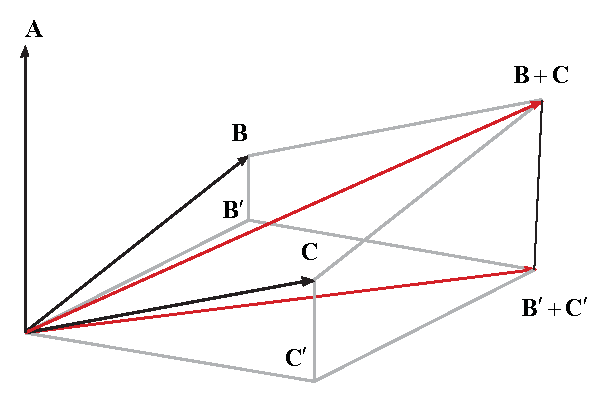
\includegraphics[width=8.5cm]{./figures/CrossP.pdf}
\caption{把 $\vec B,\vec C,\vec D$ 投影到与 $\vec A$ 垂直的平面上}
\end{figure}
首先令
\begin{equation}
\vec D = \vec B + \vec C
\end{equation}
把矢量 $\vec B,\vec C,\vec D$ 在与矢量 $\vec A$ 垂直的平面上投影,分别得到 $\vec B',\vec C',\vec D'$. 显然,$\vec D'=\vec B'+\vec C'$. 

现在先证明
\begin{equation}
\vec A \cross \vec B = \vec A \cross \vec B'
\end{equation} 
这是叉乘的一个基本的性质.首先,
根据叉乘的几何定义\upref{Cross}, $\vec A \cross \vec B$ 与
 $\vec A \cross \vec B'$ 的方向相同.另外
\begin{equation}
\abs{\vec A \cross \vec B}  = \abs{\vec A} \abs{\vec B} \sin{\theta_{AB}} = \abs{\vec A} \abs{\vec B'}=\abs{\vec A \cross \vec B'}
\end{equation}
所以二者模长也相等,证毕.

同理有 
\begin{equation}
\vec A \cross \vec C = \vec A \cross \vec C'
\end{equation}
\begin{equation}
\vec A \cross \vec D = \vec A \cross \vec D'
\end{equation}
所以,要证明
\begin{equation}
\vec A \cross \vec D = \vec A \cross \vec B + \vec A \cross \vec C
\end{equation}
只需要证明
\begin{equation}
\vec A \cross \vec D' = \vec A \cross \vec B' + \vec A \cross \vec C'
\end{equation}
即可.

由于 $\vec B', \vec C', \vec D'$ 都与 $\vec A$ 垂直,所以 $\vec A$ 与之叉乘的效果相当于 $\vec B', \vec C', \vec D'$ 的模长分别乘以 $\abs {\vec A}$, 且绕 $\vec A$ 逆时针分别旋转 $90°$. 所以上式就是在说,“ $\vec D'$ 乘以 $\abs{\vec A} $ 旋转90°”和“ $\vec B'$ 与 $\vec C'$ 分别乘以 $\abs{\vec A}$ 旋转90°再相加”结果相同,而这显然成立. 证毕.




















